\documentclass[pdf,color]{UoBnote}

\author{Rahim Topadar}

\shorttitle{Group Studies Report}
\title{Group Studies Report}
\date{\today}
%\issue{1}
\usepackage{float}
\usepackage[labelformat=empty]{caption}


\begin{document}
\maketitle
\tableofcontents
\vspace{1cm}\hrule \vspace{1cm}
%\newpage



\section{Exposure Times}

The main aim of this project is to produce an observing strategy to view some of the earliest galaxies in the universe. An important aspect of this is therefore the viewing of the galaxies themselves and the time it will take to do so. The time required to view these galaxies depends not only on the telescope being used, but also the devices used. A charged coupled device (CCD) will be used to measure the light from these sources and so to calculate the times required to view these galaxies, these must be understood in more detail. The telescope or telescopes used during the observation of these galaxies will have different properties which will affect the time required to view the source. Some of these are discussed below.

\subsection{Telescope Properties}
\subsubsection{Mirror Reflectivity}
One such factor that will increase the time required to view a source is the reflectivity of the mirrors used on the telescope. The mirror reflectivity, given as a percentage, is the amount of light reflected by the mirror. Some of the light is absorbed as the mirror is not one hundred per cent efficient meaning not all photons striking the mirror reach the CCD. The reflectivity differs depending on the material used on the surface of the mirrors. Various optical coatings are produced and used depending on the wavelengths being observed, for example, the James Webb Space Telescope uses a gold coating which is particularly useful in the infrared region and also very durable due to the inert nature of Gold. The reflectivity of this gold coated mirror is in the region of 98\% - 99\% [1]. Other coatings regularly used include aluminium, which has a reflectivity in the region of 80\% - 90\% and is utilised in the UV and IR range, as well as silver, which has a reflectivity in the range of 95\% - 99\% and is utilised in the visible and IR range.

\subsubsection{Telescope Throughput}
The definition of throughput is the ratio of the flux detected by a particular instrument in a given filter and the incoming flux measured over an area equal to the area of the telescope primary mirror [2]. The throughput is therefore the percentage of photons striking the primary mirror that reach the CCD and are recorded. This contributes to the time required to observe a source as not all the photons striking the primary mirror, originated from the source, will reach the CCD. As the number of photons reaching the CCD is fewer, a larger portion of time is required to obtain the sought after signal-to-noise ratio and so the overall observation lasts a longer period of time.

\subsubsection{Filters}
An astronomical filter is used on telescopes to remove light of unwanted wavelengths above and below a certain bandpass where a bandpass is a range of wavelengths that can pass through the filter. The width of this bandpass is commonly known as the bandwidth and is commonly used in astronomical calculations. The filter used will contain the specific wavelength being observed within the bandpass and reduce flux from other parts of the spectrum. A narrower filter will therefore ensure less background flux is observed reducing the error on the number of photons arriving from the source.\\
\newline
A filter is usually denoted with the central wavelength and width of the filter. For example, one particular filter used on the James Webb Space Telescope is named F160N, denoting a central wavelength of 1.6μm and a narrow bandwidth. The bandwidth can then be found as it will be specific to the filter. \\
\newline
The filter used is dependent on the redshifted wavelength of light from the source being observed. The wavelength of the redshifted light will be matched to a filter with the closest central wavelength to this wavelength. The bandpass of the telescope is the range of wavelengths that can pass through the filter and be measured as flux and so matching the redshifted wavelength to a filter with a similar central wavelength will allow the most flux from the source to be measured.


\subsubsection{Field of View}
The Field of view is specific to each telescope and gives the area of sky that is subtended by the CCD. This therefore depends on the CCD and the angle of sky subtended by each pixel. From this, the total area of sky imaged on the CCD can be determined. This is an important factor to take into account during the final observing strategy as, although a particular telescope may be quicker in finding a source, a larger field of view will mean more galaxies can be viewed. This therefore means a compromise must be produced to develop the optimum observing strategy.\\

\subsection{Charged Coupled Devices}
A charged coupled device or CCD is currently the detector of choice in astronomy and is used to produce images using incoming photons. A CCD works over a broad range of wavelengths and generally has high quantum efficiency within this range. They can vary in size from 1.3mm to up to 70mm across the diagonal. A larger size means more photosites and usually better image quality however the price of a CCD unfortunately rises exponentially with size ranging from \$60 to \$4000. They are still regarded as the best detectors available to astronomers and so are widely used in astronomical observations.\\
\newline
CCDs consist of an array of metal-oxide semiconductor (MOS) capacitors, known as photo-detector junctions or photosites, formed on a silicon substrate. One pixel in the CCD can contain between one and a few of these capacitors. Each photosite contains a charge isolated from other photosites by a voltage applied through conductive channels on the surface of the silicon [3]. The MOS capacitor is formed by structured with a metal electrode applied on top of a silicon substrate usually separated by a thin layer of insulation. At the beginning of each exposure, the electrodes are positively charged repelling holes in the substrate forming a depletion region which is an electrostatic potential well. Photons entering the substrate free electrons via the photoelectric effect and these are then attracted to the positively charged electrode and so are collected in the depletion region. The holes generated are repelled away from the depletion region and are lost in the substrate. The electrons generated can then be collected in the pixel and are counted to reproduce the pattern of the incident light producing an image.\\
\newline
The photosites on a CCD are arranged in columns and lines convenient for the readout procedure. The array contains a special row of photosites on the bottom line known as the serial register. Upon completion of the exposure, the electrons in the columns of the array are clocked down one line with the bottom line entering the serial register. The serial register is then clocked into a charge detection node moving one pixel at a time. The electrons move along the row towards the charge detection node and upon completion of clocking each row, the next row up will drop into the serial register and be clocked in an identical fashion [4]. During this readout procedure, a shutter must be applied to prevent light generating further electrons. The readout time of a CCD can vary from a fraction of a second to around ten seconds.\\
\newline
The CCD does however have numerous errors known as noise, which contribute to the integration time required to view these early galaxies and so must be taken into account. The conversion of light to pixel values in a CCD leads to an inevitable noise being introduced into the image. This noise is the unwanted variations in pixel values and causes the image produced to differ from the one being observed. The noise incurred will make it more difficult to distinguish the source being observed hence increasing the integration time. For an electrical measuring system such as a CCD, a signal to noise ratio characterises the quality of the measurement taken where the signal to noise ratio ($\frac{S}{N}$) is the ratio of signal from the source being observed and signal produced by background radiation and other sources of noise. This is generally used to quantify the quality of a CCD measurement. The main sources of noise for a CCD are the dark current, sky background and read noise, which are all described below.

\subsubsection{Poisson Error}
The Poisson error ($\sigma$$_{Poisson}$) or photon counting error is due to variations in the incoming flux of a source. As the photons from the source arrive randomly, the actual number arriving at a certain time or in a small time interval may differ from the average and so the error is on the detection of these photons. The Poisson error can be calculated quite simply as the error is the square root of the number of counts. This is shown below where $\it{F}$ is the incoming flux and t is the exposure time.\\
\begin{equation}
\sigma_{Poisson} = \sqrt{Ft}
\end{equation}

\subsubsection{Dark Current}
Dark current ($\sigma$$_{Dark}$), also known as thermal current, is due to the random generation of electrons and holes within the substrate of the MOS capacitor. Atoms in the silicon substrate of the CCD used are thermally excited and thus electrons are freed. These are then counted along with the electrons freed by photons from the object being observed. This occurs even when the CCD is not exposed to light, hence there is a steady creation of electrons, and this is called the dark or thermal current. As this is caused by thermal excitation, it strongly depends on the temperature at which the device is operating. At any given temperature, the rate at which electrons are freed is constant, however for every rise in temperature of 6 degrees Celsius, the dark current produced approximately doubles [5]. This relationship is shown in figure - below [6].

\begin{figure}[H]
\begin{center}
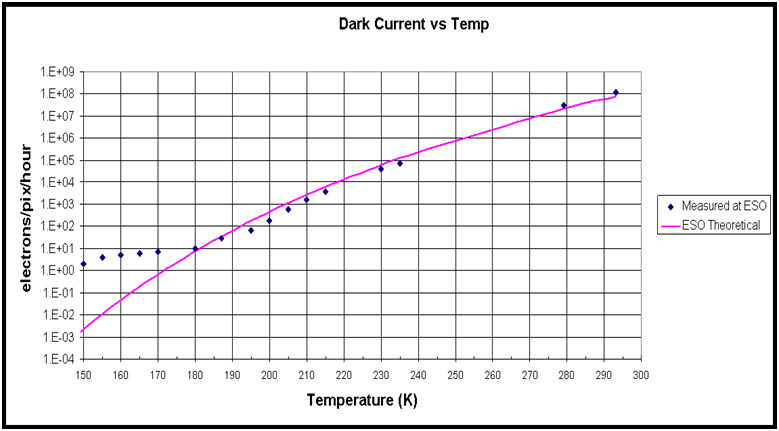
\includegraphics[scale=0.61]{Dark.png}
\end{center}
\caption{A graph showing the relationship between dark current and temperature}\label{fig:figure1}
\end{figure}
\noindent
Figure 1 shows that relationship between temperature and dark current for a custom designed CCD provided to the European Southern Observatory and shows clearly the increase in dark current at higher temperatures. CCD’s are therefore cooled, often with the use of liquid nitrogen, to minimise this effect. The dark current itself is a relatively small electric current that flows through numerous photosensitive devices, and is one of the main sources of noise for a CCD. The dark noise contributed to the total noise can be calculated using the formula below where $\it{D}$ is the dark current in electrons per second per pixel, $\it{t}$ is the exposure time in seconds and N$_{pix}$ is the number of pixels in the CCD aperture.\\
\begin{equation}
\sigma_{Dark} = \sqrt{DNt}
\end{equation}
\subsubsection{Read Noise}
When the electrons accumulated by the CCD are being read or clocked off and converted to a voltage, a readout noise ($\sigma$$_{RN}$), a small, random variation generated by the CCD’s charge detection node is added. This noise is expressed as a number of electrons per second per pixel and is a fundamental trait of CCD’s. It will, unfortunately, occur in all CCD’s, from ones used in simple webcams to those used on the Hubble Space Telescope [7]. The read noise contributed to the total noise can be calculated using the formula below where $\it{R}$ is the read noise of the CCD in electrons and N$_{pix}$ is the number of pixels in the CCD aperture.\\
\begin{equation}
\sigma_{RN} = R\sqrt{N}
\end{equation}

\subsubsection{Sky Background}
YOU ALREADY HAVE THE LATEST VERSION OF THIS SECTION. PLEASE JUST ADD THIS AT THE END.\\
The total sky background is measured to be $\it{B}$ photons per second per pixel and the noise contributed can be calculated using the formula below where $\it{t}$ is the exposure time and N$_{pix}$ is the number of pixels in the CCD aperture.\\
\begin{equation}
\sigma_{Sky} = \sqrt{DNt}
\end{equation}
\subsubsection{Signal-to-noise Ratio}
The quality of a CCD image is quantified by a signal-to-noise ratio which can be established from the source signal and all noise contributions. The different types of noise discussed above, all contribute to a total noise ($\sigma$) in the received signal which can be calculated using the equation below:\\
\begin{equation}
\sigma^{2} = \sigma_{Poisson}^{2} + \sigma_{Dark}^{2} + \sigma_{Sky}^{2} + \sigma_{RN}^{2}
\end{equation}
\newline
 As the CCD is exposed to incoming light, both the background and the source signal build up. The background is randomly and evenly distributed and so also contributes to the peak of the signal which therefore sits as a peak or peaks above a layer of background and so can be distinguished. This can be seen on figure – below where B is labelled in the region of background [15]. \\
\newline
\begin{figure}[H]
\begin{center}
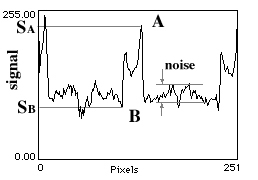
\includegraphics[scale=0.61]{SNR.png}
\end{center}
\caption{The accumulation of signal, background and noise}\label{fig:figure1}
\end{figure}
\noindent
\newline
The signal-to-noise ratio is therefore the total number of photons from the source reaching the CCD divided by the total noise for a given exposure time. As the exposure time increases, both signals, from source and background, cause an increase in counts establishing the signal more clearly. The signal-to-noise ratio is therefore also dependant on the exposure time although it is common for astronomers to decide on a signal-to-noise ratio to be obtained before calculating an exposure time.\\
\begin{equation}
\frac{S}{N} = \frac{Ft}{\sigma} =\frac{Ft}{\sqrt{\sigma_{Poisson}^{2} + \sigma_{Dark}^{2} + \sigma_{Sky}^{2} + \sigma_{RN}^{2}}}
\end{equation}
\newline
Either the signal-to-noise ratio or exposure time can then be calculated using the equation shown below commonly known as the CCD equation.\\
\begin{equation}
\frac{S}{N} = \frac{Ft}{\sqrt{(F + BN_{pix} + DN_{pix})t + R{^2}N_{pix}}}
\end{equation}
\newline
$\it{F}$ is the incident number of photons from the source per second, $\it{t}$ is the exposure time, $\it{D}$ is the dark current in electrons per second per pixel, $\it{B}$ is the sky background in photons per second per pixel and $\it{R}$ is the read noise in electrons. N$_{pix}$ is the number of pixels within the aperture area of the CCD and so is the number of pixels that are clocked to produce an image. This is dependent on the either the angular resolution of the telescope or the angular size of the object being observed depending on which is the limiting factor of the telescope. Observations on the James Webb Space Telescope will produce images with a signal-to-noise ratio of 10 indicating the current image quality desired.

\subsection{Calculating Exposure Time}
To calculate the exposure time required to view an object at a particular signal-to-noise ratio, the flux density of the source must first be obtained. The flux of the source incident on the CCD can be calculated using the value of apparent magnitude gained from the computational model produced by the Theory subgroup. This magnitude must first be converted to a flux per unit frequency ($\it{F_\nu}$) using equation 8.1\\
\newline
This must then be converted to flux per unit wavelength for use with the properties of the telescope as well as to the required units of J/s/cm$^2$/$\mu$m. This can be done via the formula below.\\
\newline
\begin{equation}
F_\lambda = \frac{\nu F_\nu \times 10^{-7}}{\lambda}
\end{equation}
\newline
This can then be used to calculate the number of photons striking the primary mirror of the telescope by multiplying this value of flux by the area of the telescopes primary mirror, the bandwidth of the telescope as well as the number of photons per joule of energy. The energy of each photon can be calculated using the wavelength of the incoming photon via $\it{E}$ = $\frac{\it{hc}}{\lambda}$ and the reciprocal of this value will then give the number of photons per joule of energy. The wavelength of the incoming photon is dependent on the redshift of the source via equation 15.1. The number of photons reaching the CCD can then be calculated by multiplying the number of photons reaching the primary mirror by the throughput of the filter as well as the reflectivity of each mirror the photon must reflect off before reaching the CCD. A rearranged form of the CCD equation, shown below, can then be utilised to calculate an exposure time required to view a given source.\\
\newline
\begin{equation}
F^2t^2 - (\frac{S}{N})(F + BN_{pix} + DN_{pix})t - (\frac{S}{N})R{^2}N_{pix} = 0
\end{equation}
\newline
The quadratic formula can then be used to calculate a value of exposure time $\it{t}$ in seconds. For ground based telescopes that are background limited, i.e. they receive more photons from background than from the source, this calculation of exposure using the CCD equation can be slightly simplified to:\\
\newline
\begin{equation}
t = (\frac{S}{N})^2 \frac{BN}{F^2}
\end{equation}
\newline
A program was created to complete these calculations incorporating the above equations for various sources and provide the exposure times required for numerous telescopes. These values were then used to determine the suitability of the numerous telescopes for observing high redshift galaxies from the start of the epoch of re-ionisation along with galaxies formed at the end of the EoR. These exposure times calculated are the time required to produce an image with a certain signal-to-noise ratio in one band and so a further 2 or 3 observations must be taken in different bands to confirm the redshift of the galaxies via the dropout method.

\subsection{Overhead Times}
There are many factors that contribute to the time required with a telescope to view a chosen object. Time required with the shutters of the telescope closed is regarded as an overhead time and must be considered during the final observational strategy. This includes time for each of the following [16]:
\begin{itemize}
\item Telescope Alignment
\item Changing filters. This usally requires a time of around 1 minute however this may differ for different instruments.
\item Changing CCDs to avoid loss of data due to cosmic ray events. Cosmic ray events contribute photons that contaminate pixels in the CCD meaning the image is also slightly contaminated. To avoid this, exposure time is normally split up into a number of separate exposures thus minimising the contamination due to cosmic rays. This can normally be set using a CR-SPLIT option which allocates a fraction of the exposure time to each exposure[17]. Importantly, cosmic rays have less impact during observations of small targets such as the galaxies being observed during this project. The splitting of the total exposure time into separate exposures also means an overhead time to replace the CCDs must be considered during the final observing strategy.
\item Clearing the CCD. The CCD is cleared before every exposure and takes approximately 16 seconds.
\item Readout of the CCD. The readout time for a CCD is generally around one minte but increases for exposures of longer than 180 seconds. This readout time is for one CCD and so must be multiplied by the number of CCDs used  during the exposure. The number of exposures will be increased if the CR-SPLIT option is used.
\item Dithering. This is the use of small movements to allow for better removal of chip defects.
\item Transmission of data to Earth from a space based telescope
\end{itemize}
\noindent
Overhead times are extremely difficult to determine quantitatively with times for each of these overheads varying considerably depending on circumstance and the instrument or telescope used. During the final observational strategy for this project, an additional overhead time of 10\% of the required exposure time will be allocated. \\

\section{Ground Based versus Space Based Telescopes}
Ground based telescopes and space based telescopes have distinct advantages and disadvantages over one another and these must be considered when deciding which telescope or telescopes to use as part of the final observing strategy. This section looks at these advantages and disadvantages whilst also looking to the future for new developments which could prove useful to the overall project.\\
\newline
Ground based telescopes are seeing limited which is a resolving limitation due to distortion caused by the atmosphere. Light is scattered by the atmosphere and so detecting a source by these telescopes can be difficult. This is discussed further in chapter ASTRONOMICAL SEEING. There is also the limitation of considerably more background light, compared to what is measured by space telescopes. To minimise these limitations, ground based telescopes are usually located at high altitude at locations such as Mauna Kea, Hawaii or Cerro Paranal, Chile. The main advantage of ground based telescopes however is that they can be built to very large sizes with telescopes with a primary diameter of around 30metres on the periphery. This cannot be achieved by space telescopes as the cost of transport to space would be very large and the telescope may well be damaged during this transportation. This also provides the ground based telescopes with very large fields of view meaning they can see more of the sky in a single observation. Importantly, they are also much cheaper to build and maintain.\\
\newline
Space based telescopes are diffraction limited, i.e. the main limitation is whether the angular resolution of the telescope can resolve the object being observed. Light arriving from the source is diffracted at the telescopes aperture spreading out the light. This subtends to an angle and becomes the minimum angle that the telescope can resolve. This is important as light from other sources in the sky may almost overlap and so this diffraction limited angle gives the angle in the sky which can be resolved. Thus if the diffraction angle is small, the better the resolving power of the telescope. Should two sources fall within this diffraction angle when looking into the sky, the telescope will not be able to resolve the two objects and so one cannot be distinguished from another. The angular resolution of the telescope can be calculated according to the Rayleigh criterion below where $\lambda$ is the wavelength of the incoming photon and $\it{D}$ is the primary mirror diameter of the telescope.\\

\begin{equation}
\Delta\theta= \frac{(1.22 \lambda)}D
\end{equation}
\newline
This also shows that the larger the diameter, the smaller the diffraction angle will be and so the better the telescope will be at resolving sources. This gives space based telescopes a distinct advantage over ground based telescopes as the seeing limitation of ground based telescopes often means that the diffraction angle is superseded. The source blurred by the atmosphere has a much greater spreading of light and so the smallest angle that it is possible to resolve is therefore much larger meaning the telescope will not be as effective when looking at distant sources. Other advantages of space based telescopes include receiving considerably less background light and that they can be operated for longer time periods during the day whereas ground based telescopes cannot be used for observations during the daytime or in adverse weather conditions such as a cloudy sky.\\
\newline
The main disadvantage of space based telescope is that they are vastly more expensive to build and maintain and must also be transported into space. This is usually done with the aid of a rocket and so the cost of achieving this can be considerable. The telescope may also be damaged during this transportation and so this limits the size of the telescope as a smaller size will mean a smaller chance of being damaged. The James Webb Space Telescope scheduled for launch in 2018 consists of a 6.5 metre primary mirror made up of multiple mirrors that will unfold once it is in space. Despite this folding up of the telescope, the primary mirror size is still small relative to some ground based ones currently in use such as the VLT (primary mirror of 8.2 metres) and is considerably smaller than some proposed for the future such as the EELT (primary mirror 39.3 metres). \\

\subsection{Astronomical Seeing}
Plane waves from a source being observed are distorted by the Earth’s atmosphere and so upon reaching a telescope within the atmosphere are slightly perturbed and the image formed, blurred. This effect is contributed to by numerous layers where different temperatures or the interaction of different wind speed causes this effect with ‘Seeing’ the term used to describe the total distortion of the wavefront [18]. This effect is shown below in figure - where a turbulent layer of the atmosphere causes a change in the shape of the wavefront. This turbulence is caused by micro-thermal fluctuations which can be caused by a variety of reasons such as friction encountered by air flow at the Earth’s surface or differential heating of the Earth’s surface [19].\\
\newline
\begin{figure}[H]
\begin{center}
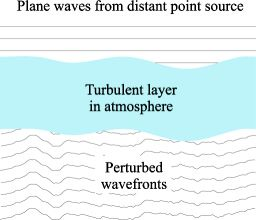
\includegraphics[scale=1.0]{Seeing.png}
\end{center}
\caption{The perturbation of a wavefront due to the atmosphere [20]}\label{fig:figure1}
\end{figure}

\noindent
Whilst the resolving power of a telescope is generally largely dependent on its diameter, this seeing limitation becomes the major source of error when resolving a point source from within the Earth’s atmosphere. This is consequently the main limitation for ground based telescopes which are therefore known as being seeing limited. A point spread function (PSF) imaged in these circumstances produces what is known as a seeing disc due to the atmospheric turbulence and the most common measurement used to describe this effect is the full width at half maximum (FWHM), shown below in figure - where a peak shape is produced by this overall blurring of the source. When measuring the flux arriving at the CCD from a particular source, an area of radius four times the FWHM is recorded over and so a larger value of FWHM also increases the integration time required to observe the source. \\
\newline
\begin{figure}[H]
\begin{center}
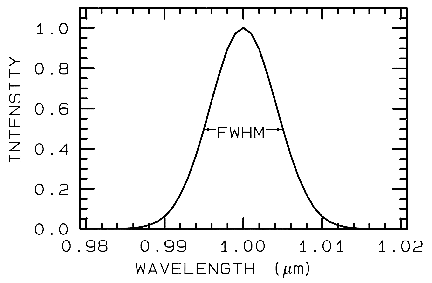
\includegraphics[scale=0.9]{FWHM.png}
\end{center}
\caption{A peak produced by the blurring of a point source [21]}\label{fig:figure1}
\end{figure}
\noindent

\subsection{The Future of Ground Based Telescopes}
The main disadvantage of ground based telescopes compared to space based telescopes is the poorer resolution due to the distortion caused by the atmosphere or astronomical seeing. The introduction of adaptive optics however, should help resolve this issue and allow ground based telescopes to be only diffraction limited similar to space based ones. This, combined with the large diameter mirrors currently in the pipeline such as for the European Extremely Large Telescope (E-ELT), a primary mirror of 39.3 metres, and the Giant Magellan Telescope (GMT), a primary mirror of 25 metres, ensure ground based telescopes hold a place in the future of space observation, even if just to compliment space based ones. The larger mirrors ensure a greater light collecting power, receiving more photons for the source being observed and so significantly reducing the observing time required. These large diameter mirrors are currently only possible for ground based telescopes and so provide them with a distinct advantage over space based ones. \\

\subsubsection{Adaptive Optics}
As described earlier in astronomical seeing, light passing through the atmosphere from a source, such as a distant galaxy, is perturbed due to atmospheric turbulence and so the images produced by ground based telescopes are blurred. Adaptive optics works by first sensing the wavefront perturbations and then counteracting this blurring in real time thus enabling the telescopes to hold a much larger resolving power. This is usually done with light from a guide star although as sufficiently bright natural guide stars are not readily available, it is possible to use a laser guide stars produced at the observatory. This system will be used on future ground based telescopes ensuring they are no longer limited by the ability to resolve a source. An example of how this is set up, as on the Subaru Telescope, is shown below in figure -. \\
\newline
\newline
\begin{figure}[H]
\begin{center}
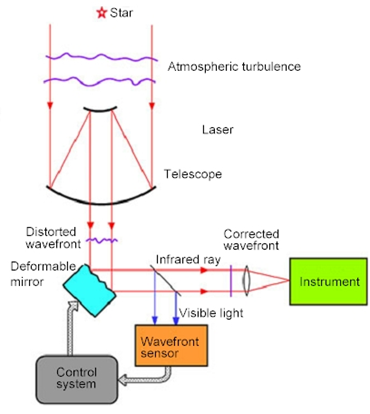
\includegraphics[scale=1]{AdaptiveOptics.png}
\end{center}
\caption{A schematic of an adaptive optics system [22]}\label{fig:figure1}
\end{figure}
\noindent
The wavefront sensor (WFS) measures the distortions in the incoming wavefront of light. This then provides the measured information to an actuator control computer identified in figure - as the control system. This then adjusts the shape of the adjustable mirror to effectively correct the wavefront reaching the telescope [23].  The wavefront sensor can measure the distortions introduced into the wavefront on the timescale of a few milliseconds with the information then computed and the shape of the mirror adjusted accordingly. The correction process should therefore be completed in a time similar to the time between the changes of the wavefront thus ensuring the distortion is compensated for.\\

\section{References}

Hey Josh/Lewis, References 8 - 14 in the sky background section which has already been submitted, the rest are listed below. A lot are from the same two books but i referenced them again. Feel free to change what you need to. Every section included here has been updated so please replace the ones i previously submitted.\\
\newline
\noindent
1. http://www.quantumcoating.com/fsg98.asp
%@misc{quantum_coating,
%  author 		= {Quantum Coatings Incorporated},
%  title 		= {{Gold - FSG98 and more!}},
%  howpublished  = "\url{http://www.quantumcoating.com/fsg98.asp}",
%  year 			= {2013},
%}
\\
2. http://www.cfht.hawaii.edu/Instruments/Imaging/WIRCam/WIRCamThroughput.html
%@misc{Canada_France_Hawaii_throughput,
%  author 		= {Canada-France-Hawaii Telescope},
%  title 		= {{WIRCam Throughput}},
%  howpublished  = "\url{http://www.cfht.hawaii.edu/Instruments/Imaging/WIRCam/WIRCamThroughput.html}",
%  year 			= {2013},
%}
\\
3. Diffraction-Limited Imaging with Large and Moderate Telescopes, pgs 331 - 333
%@book{Saha,
%       author = {Swapan K Saha},
%        title = { Diffraction-Limited Imaging with Large and Moderate Telescopes},
%    publisher = {World Scientific Publishing Co. Pte. Ltd.},
%         year = "2007",
%}
\\
4. The handbook of Astronomical Image Processing, Richard Berry \& James Burnell, page 16
%@book{Images,
%       author = {Richard Berry & James Burnell},
%        title = {The handbook of Astronomical Image Processing},
%    publisher = {Willmann-Bell; 1 edition},
%         year = "2000",
%}
\\
5. The handbook of Astronomical Image Processing, Richard Berry \& James Burnell, pages 124-125
%@book{Images,
%       author = {Richard Berry & James Burnell},
%        title = {The handbook of Astronomical Image Processing},
%    publisher = {Willmann-Bell; 1 edition},
%         year = "2000",
%}
\\
6. http://www.eso.org/sci/facilities/develop/detectors/optdet/docs/reports/EEV-report.html
%@misc{throughput,
%  author 		= {European Southern Observatory},
%  title 		= {{EEV44-82 CCDs Performance overview}},
%  howpublished  = "\url{http://www.eso.org/sci/facilities/develop/detectors/optdet/docs/reports/EEV-report.html}",
%  year 			= {1999},
%}
\\
7.	http://www.qsimaging.com/ccd\_noise.html
%@misc{Understanding_CCD_Read_Noise,
%  author 		= {QSI},
%  title 		= {{Understanding CCD Read Noise}},
%  howpublished  = "\url{http://www.qsimaging.com/ccd_noise.html}",
%  year 			= {2008},
%}
\\
15. http://www.emal.engin.umich.edu/courses/sem\_lecturecw/SEM\_SignalNoise.html
%@misc{SNR,
%  author 		= {Electron Microbeam Analysis Laboratory},
%  title 		= {{Signal to Noise Ratio}},
%  howpublished  = "\url{http://www.emal.engin.umich.edu/courses/sem_lecturecw/SEM_SignalNoise.html}",
%  year 			= {2007},
%}
\\
16.	http://documents.stsci.edu/hst/wfpc2/documents/handbooks/cycle17/ch2\_instrument8.html\#440922
%@misc{noise,
%  author 		= {Space Telescope Science Institute},
%  title 		= {{Overhead Times}},
%  howpublished  = "\url{http://documents.stsci.edu/hst/wfpc2/documents/handbooks/cycle17/ch2_instrument8.html#440922}",
%  year 			= {2008},
%}
\\
17.	http://documents.stsci.edu/hst/wfpc2/documents/handbooks/cycle17/ch7\_strategy5.html\#442816
%@misc{noise,
%  author 		= {Space Telescope Science Institute},
%  title 		= {{Cosmic Rays}},
%  howpublished  = "\url{http://documents.stsci.edu/hst/wfpc2/documents/handbooks/cycle17/ch7_strategy5.html#442816}",
%  year 			= {2008},
%}
\\
18. Diffraction-Limited Imaging with Large and Moderate Telescopes, pg 188
%@book{Saha,
%       author = {Swapan K Saha},
%        title = { Diffraction-Limited Imaging with Large and Moderate Telescopes},
%    publisher = {World Scientific Publishing Co. Pte. Ltd.},
%         year = "2007",
%}
\\
19. Diffraction-Limited Imaging with Large and Moderate Telescopes, pg 161
%@book{Saha,
%       author = {Swapan K Saha},
%        title = { Diffraction-Limited Imaging with Large and Moderate Telescopes},
%    publisher = {World Scientific Publishing Co. Pte. Ltd.},
%         year = "2007",
%}
\\
20. www.optcorp.com
%@misc{Seeing,
%  author 		= {Oceanside Photo & Telescope},
%  title 		= {{Astronomical Seeing}},
%  howpublished  = "\url{http://www.optcorp.com/edu/articleDetailEDU.aspx?aid=2250}",
%  year 			= {2008},
%}
\\
21. http://web.williams.edu/astronomy/Course-Pages/402/FWHM.gif
%@misc{FWHM,
%  author 		= {Williams},
%  title 		= {{FWHM}},
%  howpublished  = "\url{http://web.williams.edu/astronomy/Course-Pages/402/FWHM.gif}",
%  year 			= {2007},
%}
\\
22. http://www.nalux-world.com/subaru\_e.php
%@misc{Adaptive,
%  author 		= {Nalux},
%  title 		= {{SUBARU Telescope}},
%  howpublished  = "\url{http://www.nalux-world.com/subaru_e.php}",
%  year 			= {2013},
%}
\\
23. Diffraction-Limited Imaging with Large and Moderate Telescopes, pages 271-272
%@book{Saha,
%       author = {Swapan K Saha},
%        title = { Diffraction-Limited Imaging with Large and Moderate Telescopes},
%    publisher = {World Scientific Publishing Co. Pte. Ltd.},
%         year = "2007",
%}
\end{document}
